\part{Part Two}

\chapter{学习OMNeT++Map}

\begin{summary}
欢迎来到第三章,本章主要介绍OMNeT++官方已经提供的学习资料有哪些,并以OMNeT++内一系类tictoc作为实例进行简单的设计说明,通过本章你可以快速的了解到如何学习OMNeT++、掌握官方的学习资料和利用OMNeT++可以做哪些事情。\\ \\
\end{summary}

\section{学习map}
就目前学习OMNeT++的资料来说,网上的资料有:
\begin{itemize}
	\item 《 OMNeT++中文使用手册》
	\item 《 OMNeT++与网络仿真》
	\item 《 OMNeT++网络仿真》 
\end{itemize}

目前较全的资料就上面三种,其中前两种参考价值比较好一些,其中第一本就是OMNeT++官方提供的资料的翻译版,主要介绍范范的仿真程序设计,不能称其为学习教程,应该叫参考资料。第二本《 OMNeT++与网络仿真》与第一本相比,在仿真程序的设计时更有价值一些,对部分函数接口有介绍,但是没有给出使用场景。其实到目前,作者认为还是官方提供的入门手册对初学者较友好一些,但是问题在于初学的时候我们不知道它的存在,包括我在初学的时候也是恍恍惚惚的,为了使读者在初学的时候就更好的利用这些资料,我在这里总结出官方到底提供了哪些资料。\\ \\

\subsection{OMNeT++文档与指导书}
在OMNeT++安装路径下,官方提供了较多的使用指南,大多数以网页的形式给出。第一个要介绍的就是包括安装手册在内的多个文档入口:

\begin{itemize}
\item 路径:\url{omnetpp-5.2/doc/index.html}
\end{itemize}

其内容包括从软件安装、初学Tictoc多个仿真例子、API参考到提升篇:IDE自定义指南和并行仿真指南等,详细如下:\\

介绍、指导手册
\begin{itemize}
\item 安装指导
\item IDE 浏览
\item TicToc指导手册
\end{itemize}

文档
\begin{itemize}
	\item 仿真手册
	\item IDE用户指南
	\item API参考书
\end{itemize}

其他
\begin{itemize}
	\item IDE开发者指导
	\item IDE自定义指南
	\item 并行仿真指南
	\item NEDXML接口函数 
\end{itemize}

这里都是以中文的形式展现出官方提供的资料目录,而原目录都是以英文的形式给出。\\

\subsection{tictoc指导手册}
tictoc相当于程序中的hello world级别的例子,初学OMNeT++一般通过仿真修改tictoc例子,其路径在软件的安装路径下,点击该路径下的index.html:

\begin{itemize}
	\item 路径:omnetpp-5.2/doc/tictoc-tutorial/index.html 
\end{itemize}

包括的内容如下:
\begin{itemize}
	\item 开始:一个简单的仿真模型(**tictoc1.ned txc1.cc omnetpp.ini**)
	\item 仿真程序的执行和仿真
	\item 改进两个节点仿真模型(**tictoc9.ned txc9.cc omnetpp.ini**)
	\item 一个复杂的网络(**tictoc13.ned, tictoc13.msg, txc13.cc, omnetpp.ini**)
	\item 如何添加统计量(**tictoc17.ned, tictoc17.msg, txc17.cc, omnetpp.ini**)
	\item 如何可视化观察仿真结果
	\item 如何添加参数 (**在omnetpp.ini中配置.ned文件需要的参数**)\\
\end{itemize}

对于以上资料是目前入学OMNeT++较全系统的资料,从工程搭建、调试到添加统计量这些都是实际的网络仿真程序中一般会用到的,比如统计量,一般在网络中包括端到端延迟、入队排队时间、丢包数等。最后的仿真结果可视化观察,OMNeT++仿真程序结束后,在out文件下会生成仿真结果文件,OMNeT++提供可视化工具观察程序中统计的变量,可以转换成直方图和折线图,在后续会详细说明如何使用OMNeT++提供的观察和分析仿真结果工具。\\

\subsection{仿真手册}
官方也提供了一个较详细的仿真手册,这里还是介绍一下这个手册。\\

\begin{itemize}
\item 路径:omnetpp-5.2/doc/manual/index.html

SimulationManual仿真手册提供了设计一个OMNeT++工程各方面详细的介绍,从某种意义上来说,本手册也许就是Simulation Manual手册的一个子集,但是为了使本手册的意义更大,我将结合自己的几个月使用OMNeT++的经验,提供一些在设计网络时可能会出现的问题,以及解决办法。\\ \\
\end{itemize}

\section{个性化IDE}

添加这一节,只是个人乐趣而已,我曾经修改代码高亮花了一个下午的时间,每次总是很难找到相关的设置地方,只能说OMNeT++代码高亮设置放置的太隐秘了,到目前为止,我还是不能找到修改.ned文件的高亮设置(似乎没有这个功能)。相关.cc文件的设置地方下面会简单指明,其他更为详细的内容需要读者自行发挥。\\
\subsection{CPP高亮设置}

首先,进入到IDE设置界面:Window 》》  Preferences,如图:

\begin{figure}
	\centering
	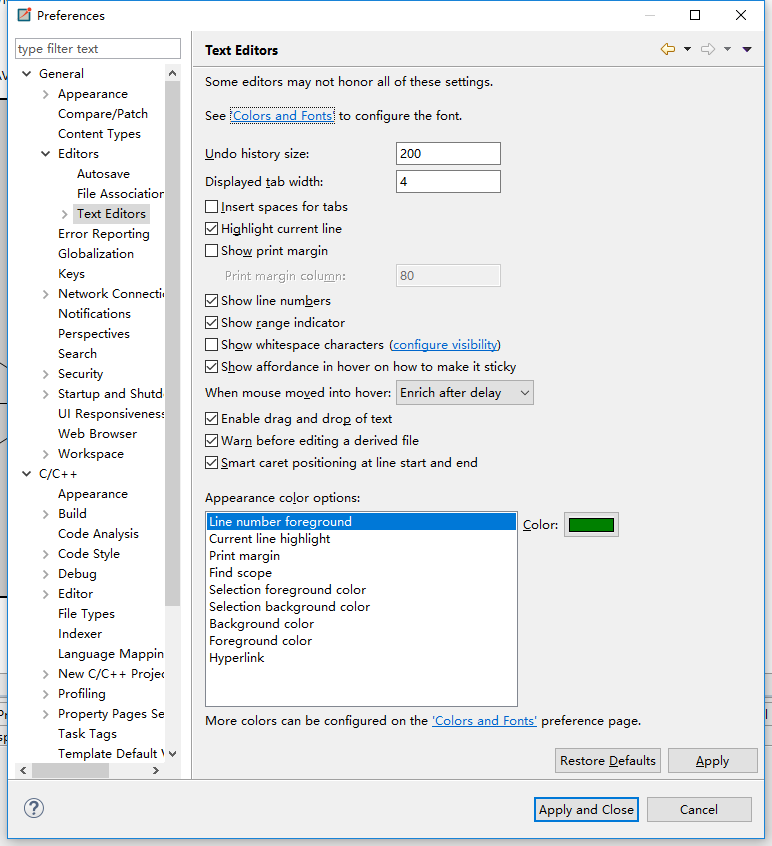
\includegraphics[width=\textwidth]{../img/chapter3/picture3-3-2.png}
	\caption{其他设置界面}\label{fig:1a}		
\end{figure}

在这一界面中,我们Tab键宽度、显示行号或者当前行背景,其他设置读者可自行编辑看看。








